\chapter{The Design and Implementation of a Verification Based Annotation System for Object Detection}
\label{chap:design} 

\section{Introduction}

This chapter describes the design and implementation of a human-in-the-loop verification based annotation system. The interface is similar to a diagram editor, however, at each step the machine model is integrated as seamlessly as possible to evaluate the easy cases and leave the annotator to verify and correct only the harder cases. 

I discuss some novel methods such as using the machine model to assist in reviewing annotations for quality assurance and also discuss a novel method for utilising weakly-confident, detected objects.

I later describe the implementation, which is written as a web application for ease of distribution and usability. The implementation is split into three parts, firstly, a web-based client, secondly, training processes running on machines with powerful \gls{GPU}s and thirdly, a server acting as an intermediary that is storing image data, user actions and parameters of trained object detection models.

\section {Goals}

The goal of any annotation system is to efficiently and accurately allow a user to annotate a set of images. The main consideration was to be of practical use for real problems. From experience gained during work on chapter~\ref{chap:bootstrap} I set out to achieve some specific goals (some developed more than others in this work):

\begin{itemize}

\item {\bf Object detection} \par
While segmentation is appropriate for some specific tasks, notably where elements of interest are irregularly shaped, object detection and variations are more generally useful. The goal is not just bounding box object detection but other annotation types such as polygons, for instance, segmentation, oriented boxes, lines and custom types of pose/keypoint estimation.

\item {\bf Verification based annotation} \par
Of methods explored in chapter~\ref{chap:bootstrap}, using human verification and correction of machine predictions seemed the most promising. Therefore the goal is to integrate this idea as seamlessly and unobtrusively as possible, 

\item {\bf Flexible use} \par
To be generally useful, a tool needs to work well in a variety of situations without needing much special tweaking. Some of the focuses in this work have been to adapt to different image resolutions, very small objects, and objects which are abundant or sparse. 

\item {\bf Easy deployment} \par
In chapter~\ref{chap:bootstrap} a C++ application was used for annotation. Two issues can be identified, firstly hardware and complex dependencies, and secondly the interactivity impairment of running GPU processes on a local machine. Along with all the dependencies required to train the model (PyTorch \cite{Paszke2017} and all its dependencies) and the \gls{GPU} requirement; it is clear that for people to use such a system a simple method for deployment is preferable. For these reasons, I focused on a web application which can run on a server with a GPU, then be accessible by anyone from anywhere.

\item {\bf Support experimentation} \par
While one goal is to reduce the amount of manual tuning necessary for most use cases, the goal is to be able to empower an annotator to get the best results from the data. This comprises  several parts: (a) the ability to get feedback, both automated in terms of testing and visual feedback on new data; (b) the ability to modify parameters, and see the results, for example, parameters change the training image size, or adding another class category; (c) to be able to organise data in useful ways, for example, to be able to filter and search, based on automated detections on new data.

\end{itemize}


Other ideas have since become more of a focus after using the system in practice, two of the most important ones being:

\begin{itemize}

\item {\bf Active learning and image selection} \par

It became apparent through experimentation (see chapter~\ref{chap:annotation} that in some dataset types, such as those where object instances are less uniform, selecting the right parts of the dataset to annotate first becomes important. Active learning also presents an opportunity to synergise with \gls{VBA}, as many images containing uncertain detections may also contain many easy to detect objects.

\item {\bf Reviewing and cross verification} \par

Given the importance of ensuring correctness in annotations, and the risk of algorithmic bias using a \gls{VBA} system (where a user may fail to correct a mistake in the machine annotated image), finding methods of validating annotations becomes important. 

\end{itemize}


\section {Verification based annotation}

At the core of the user interface is the use of an object detector seamlessly providing immediate feedback on images viewed by the user. When a previously unedited image is opened, the model provides the set of predicted detections which are presented to the user for verification. 

In the first implementation, this was a manual operation where a user viewing an image could click a button to retrieve model predictions, an unnecessary action. It does, however, make it apparent to the user where the annotations originated. One downside to the seamless detection and review interface is that it is not necessarily apparent if the annotations being viewed are the result of model predictions or previous user inputs.

\subsection{Basic operation}


\section {User interface}
\label{sec:user_interface}
 
The user interface of the system resembles a diagram editor, where annotation shapes (boxes, circles or polygons) can be drawn over an image and manipulated in the usual ways. Shapes can be moved by selecting and dragging, re-sized by scrolling the mouse wheel or by dragging control points. 

\begin{figure}[h!]
  \centering
  \includegraphics[width=1.0\linewidth]{figures/annotation/penguin_refine.pdf}
  \caption{Illustration of a human annotator refining a set of bounding box predictions. The boxes modified at each step are highlighted (corner markers shown and shaded). The image used is from the \emph{penguin dataset} \cite{PenguinData} }   
  \label{fig:penguin_refinement}
\end{figure}

An illustration of the annotation process is shown in figure~\ref{fig:penguin_refinement}, showing the user refining a set of bounding box annotations. The diagram illustrates the main operations available to the annotator, which are:

\begin{itemize}
    \item {\bf Transform bounding box}\par
An inaccurate bounding box can be corrected by clicking and dragging a corner or moving its centre by clicking on the box as a whole and dragging it. The scale may also be adjusted at the same time by scrolling the mouse wheel.
    \item {\bf Confirm weak detection}\par
If the \emph{review} mode is activated, detections of weak confidence will show with dotted lines. I use a two confidence level threshold system (see section~\ref{sec:thresholding}). A user may then click on the box to confirm it as an annotation.
    \item {\bf Delete box}\par
Any false-positive predictions from the object detector, which meets the threshold as a high confidence detection, can be deleted by selecting the box (by clicking on it) and pressing a key. 
    \item {\bf Draw box}\par
For objects in the image completely missed by the object detector, the user may draw a box by holding a key then clicking once on one corner, and again on the other corner.
    \item {\bf Change class}\par
The class of a box annotation may be changed by selecting the object and then selecting the active class. The best method for this is to set up hot-keys for some of the more commonly used classes.
    \item {\bf Submit image}\par
Once the image has been corrected to the required standard, the user may then submit the annotated image where the annotations are saved and immediately used for training.
\end{itemize}

Some of the operations above may be conflated, for example, low confidence predictions are sometimes not localised well - so the user may transform the bounding box at the same time as confirming the weak detection.


Multiple annotations can be selected together using a rectangle select and moved or deleted in one action, saving significant time when the model creates excessive extraneous detections. False positives often occur in \gls{CNN} models when an image contains objects of a scale or content outside the distribution previously seen \cite{Hendrycks2016,Lee2018}. The same property also enables adversarial attacks on \gls{CNN} classifiers. An example in the \emph{scallop} image set is seen in figure~\ref{fig:scallop_diver} where an image contains a (previously unseen) diver, leading to a selection of false positives (one of them at a high confidence detection).


\subsection {Navigation}

Navigation is crucial to being able to effectively examine an image (and thus annotate it well). The ability to zoom into a portion of an image to view it more closely and see details is important, particularly for parts of an image with higher uncertainty. Equally important is the ability to zoom out to view the whole image in order to check for missed details. 

A zooming/panning interface similar to Google Maps is provided where panning is achieved by clicking and dragging, with zooming achieved by the use of the mouse wheel. The zoom centres around the mouse cursor so that the image position at the mouse cursor is fixed under zooming.

Fitts's law is the generally accepted model to guide pointing performance where pointing time is determined by a \gls{ID} $ ID = log_2 \frac{2D}{W} $ where D is the distance to travel and W the width of the target --- having direct consequences for annotation, where the edge of a box is a narrow target for selection. 

The zooming and panning interface facilitates faster target acquisition (by reducing D and increasing W), however, in order to verify the correctness of the entire image annotation, a user must also consider the image as a whole when deciding when to submit the image. If the image has too many instances or potential instances of the target object, the risk is that the user misses some or does not remember where they have previously checked. 


\subsection {Video Annotation}

Many image datasets are either time series (for example images taken minutes apart) or are derived from video.  Approximately half the annotated datasets described in this work (see chapter \ref{chap:annotation})  are derived from video, and of those remaining, two are time series. Functionality for the annotation of video sequences is limited in this work; however, some ability to organise images in order of time (and frame sequence) was developed, and the ability to view a small amount of context in time around a current frame is supported (by use of shortcut keys).

Viewing context helps avoid ambiguity from an annotation perspective, as often in a video sequence, if something is unclear from a single frame it is possible to resolve that ambiguity by viewing back or forward in time. An example of this is in the \emph{seals} dataset (described in chapter~\ref{chap:annotation}); identifying a pup next to a mother is often somewhat ambiguous, but viewing the movement over time usually resolves the ambiguity.

Although many promising directions exist to utilise temporal and spatial consistency, for example, using tracking or interpolation between annotations, this work treats every image independently. 


\section {Which detections to show?}
\label{sec:thresholding}

Showing the right number of detections is an important factor. The consequence of showing too many or too few detections causes extra work for the annotator, either by needing to delete too many false positives or having too many boxes to draw. Object detection typically uses a confidence threshold. If the confidence is set too high, there will be many detections which would otherwise be true positives, hidden; and if set too low, the interface becomes cluttered with many false positives and hard to use.

In \cite{Fitchett2013} a method of predictive highlighting items in a file browser was shown to improve access times. When annotating an image, the missing annotations are not always prominent. A weak object detector often shows many spurious detections, and it often highlights image areas hiding more uncertain examples, acting like the predictive file highlighting effect. For this reason, I seek to make use of all the detections, even for just highlighting areas of interest to a user. 

\subsection{Making use of weak detections, dual threshold method}

 Many times, especially with difficult image detection problems, a weak detector will still produce many detections (some true positives, some false positives). The weak detector will not be able to separate these detections by confidence value. By using human verification, there are some clear strategies to separate the true positives from the false positives, while still not missing too many objects altogether. 

\begin{itemize}
    \item Set a low detection threshold and have the user delete false positives
    \item Set a low detection threshold and have the user select true positives
    \item Set a high detection threshold and have the user draw boxes around missed detections
\end{itemize}

Each of these strategies has a valid place. If detections are so noisy and if the location predictions are also very noisy (for example, when the detector is very weak, such as near the start of the process) - having the user draw boxes is often the only option. Some of these strategies are among those used by \cite{Konyushkova2017} where attempts are made to solve this problem differently, by automatically determining the best interface for a given image.

Deleting false positives is often the best option if true positives outnumber the false positives, or if the false positives are easy to select (if they are grouped, for example). Selecting true positives is often the best option if the false positives outnumber the true positives. 

Another strategy exists, which has advantages of both. Two thresholds can be used, a high confidence threshold for eliminating false positives (so that when using this threshold, the number of false positives is low), as well as a low threshold. Detections between the high and low confidence thresholds can be considered for selection as true positives (so that the number of true positives requiring selection is low).



\begin{figure}[thb]
\centering
\begin{subfigure}[t]{0.5\linewidth}
  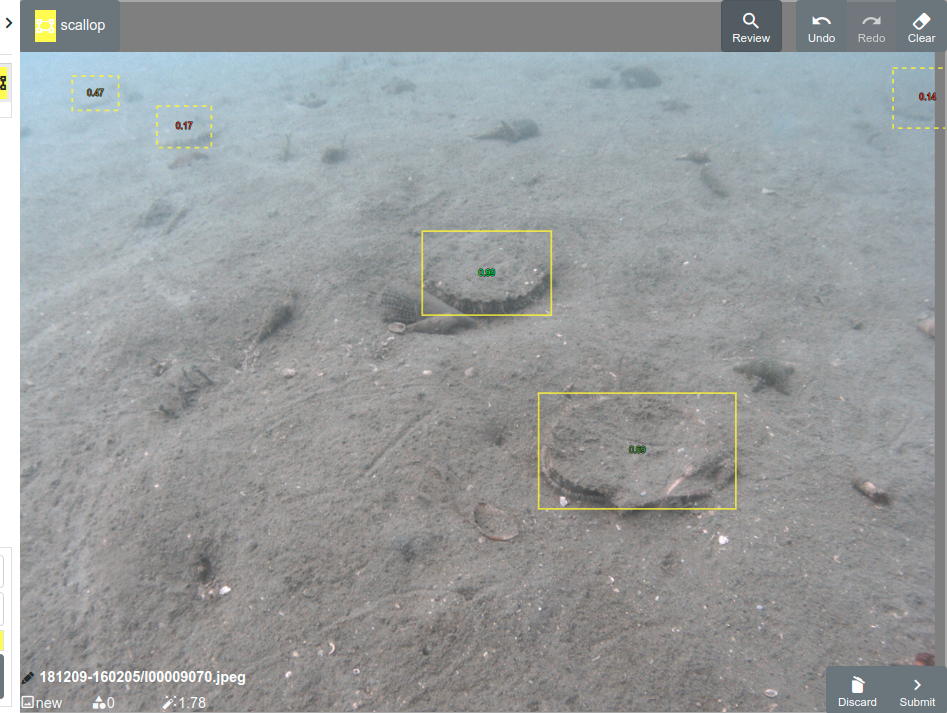
\includegraphics[width=1.0\linewidth]{figures/annotation/scallop/review_mode.png}
  \caption{}
  \label{fig:scallop_review_a}
\end{subfigure}%
\begin{subfigure}[t]{0.5\linewidth}
  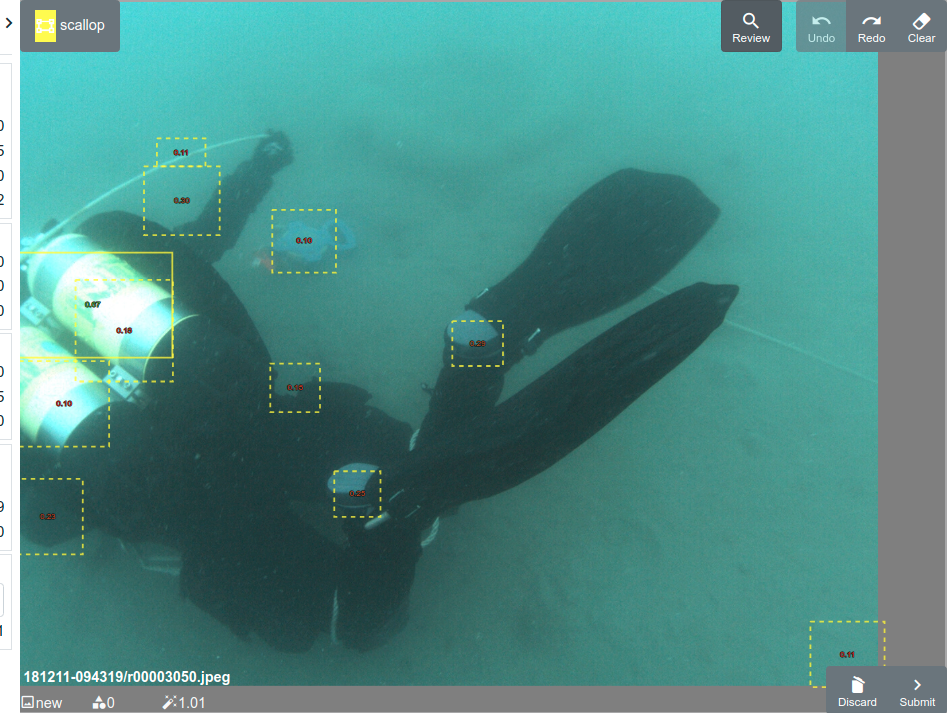
\includegraphics[width=1.0\linewidth]{figures/annotation/scallop/diver.png}
  \caption{}
  \label{fig:scallop_diver}
\end{subfigure}
\caption{Review mode used on two fresh images from the \emph{scallop} dataset, (a) showing an ideal case (b) showing an image with a high confidence false positive among low confidence detections}
\label {fig:scallop_review}
\end{figure}


I provide a key which toggles \emph{review mode} on which shows weakly confident detections which lie above a minimum threshold but below the threshold for a confident detection. When the key is held, a click is used to confirm a detection as a true positive. I term this toggle \emph{review mode}.  An example showing the use of this can be seen in figure~\ref{fig:scallop_review_a}. Where three scallops are detected in the background (with low confidence), yet are perfectly well localised, leaving the user to click on them instead of needing to draw a box.

The other advantage of this strategy is that it can bring the annotator's attention to areas of the image, which may have gone unnoticed. I have noticed in particular with the underwater scallop images, that the detector usually did a good job at bringing attention to the more uncertain scallop instances. It also provides useful feedback to the annotator of the progress of the current object detector. 

During training, it can be seen that the confidence levels provided by the object detector vary with regard to training time; this is a known property of neural network classifiers \cite{Guo2017}.

In future, I would like to investigate the calibration of thresholds using validation so that the user does not have to do this. One method is to adjust thresholds to match a specific ratio of false positives to false negatives (the desired ratio to be set by the user). Alternatively, prediction confidence itself can be calibrated to attempt to provide more consistent values. Confidence scores can be calibrated by scaling outputs prior to applying softmax normalisation \cite{Guo2017}. For object counting, I use the above method to select thresholds. In order to provide the most unbiased estimate of counts, the confidence is selected to give an equal ratio of false positives to negatives.
 
\section{Image/example selection}
\label{sec:example_selection}

While not the core focus of this work, active learning and example selection are complimentary to verification based annotation. Both attempt to remove the burden of labelling all the easy cases in a dataset. Active learning seeks to have the annotator label the most informative images by example selection, and verification based annotation attempts to achieve the same thing by automatically labelling the easy cases, so the human annotator does not have to. 

In object detection datasets, many images contain a mixture of easy and difficult examples, so it makes sense to use both active learning and a verification based annotation.  Firstly, active learning example selection picks images containing uncertain object detections. Secondly, a verification based annotation approach is taken to annotate the uncertain image, where the user needs only annotate or correct the hard cases where the model performs poorly.

I have implemented several simple metrics for selecting images based on heuristics, which I have found useful in different kinds of workflows. For example, in sparsely populated images, such as in the scallop imagery, to best utilise annotator time, it seems prudent to present images containing (or believed to contain) scallops first. Another example is annotating a single class (or few classes) from a much larger image set, where only a subset of the images contains the object in question.

Very recently, published measures of uncertainty for object detection (for example using Bayesian \gls{NMS} \cite{Harakeh}), ensembles \cite{Le2018}, or test time augmentation \cite{Wei2018}) give a future direction to integrate uncertainty approaches. Using cross-validation with an ensemble of models seems promising, although it will increase the training time.

\subsection {Image Implementation}
\label{sec:example_implementation}

Three image selection policies are implemented: (a) select images in sequence, either by time, video frame or file-name; (b) select images at random; (c) select images by a heuristic. When an image is submitted, the next image is chosen according to the policy enabled, from the set of unlabelled images (those which are not being annotated by any other user).

When example selection by heuristic is enabled, the trainer will evaluate a random sample of unseen images (images not yet annotated or discarded) for object detection at each training iteration. Object detections are then evaluated according to the heuristic and ranked for annotation ordering. 

In general, evaluating the entire image set of unlabelled images for each training iteration is usually far too slow, so using random sampling often ensures a more balanced set of training examples. Too much reliance on a heuristic may result in many similar images being selected, causing an imbalance in the training set.

For certain kinds of heuristic, such as frame variation (discussed below), it is necessary to evaluate many frames in a sequence. For this, there currently exists a manual operation where a user can schedule a full evaluation of the set of images. This evaluation can take a long time for a large image set and occurs much less frequently during the annotation process.


\subsection {Image selection heuristics}
\begin{itemize}
\item {\bf Detection score. }

Uses the sum of squares of the confidence scores, $ \sum_(p \in detections){ p^2 } $ where $p$ is the confidence for a given detection. 

    \item {\bf Count variation. } \par
Used with object counting datasets, where the sensitivity of the count in each image is used. Images with the widest difference in the count at two thresholds are selected first, the two thresholds determined on the validation set to give $ \pm 10\% $ counts.
    \item {\bf Frame variation. }  \par
In time sequence and video datasets, the variation in count between nearby frames can be used to estimate uncertainty. For this, I use the difference between a frame and a running average for a window centred around that frame. For this, the metric is determined after predictions for all frames are computed and counts estimated.
    \item {\bf Training error. }  \par
Making use of the loss from training was proposed to find training images potentially with annotation mistakes. Initial experiments with this indicate the object detection models manage to fit images, even with the most obvious mistakes, with low loss, making this form of example selection less useful. In future using a k-fold cross-validation training ensemble is proposed such that each image is left out of training for at least one model, allowing an unbiased comparison with at least that model.
\end{itemize}


\section{Browsing, sorting and reviewing images}
\label{sec:browising}


\subsection{Reviewing images}
\label{sec:reviewing}

In crowdsourcing based image annotation software, quality assurance is usually performed using cross verification. Either multiple users annotate the same images which are checked for consistency, or each image passes a set of checks performed by other users before the quality is deemed acceptable. Verification prevents malicious or incompetent users from spoiling the data and provides some assurance that the result is of high quality. In this work, I prototyped the idea of using the trained model to assist with quality assurance by (a) finding images to review (see section~\ref{sec:example_selection}), and (b) illustrating inconsistencies with the trained model.

When a previously annotated image is opened, the existing annotations are matched with model predictions, and interface functions similarly to a difference viewer (version control) for image annotations. Matches are determined by a greedy matching process as used for evaluating object detection, described in section~\ref{sec:evaluation_metrics}. The user can view these changes by toggling the \emph{review} mode on and off. This functions in a similar way to the initial refinement process where the \emph{review} mode is used to show detections of weak confidence. 

Where model predictions differ from the provided annotations, a dotted outline is shown. This highlights annotations where the localisation differs from model predictions, as well as potentially missed annotations. A confidence score is also shown on existing annotations, highlighting annotations for attention which are either missed by the model, or are potential errors in annotation.

The difficulty faced with using the trained model to determine annotation inconsistency is that the model tends to overfit the training data. In order to adequately use a trained model for this purpose, the image must not be one used directly in the training process. With the current design, this restricts the use to images in the validation set. In future, the plan is to use k-fold cross-validation, so that each image is left out of training with at least one model. 

It is anticipated that this form of quality assurance will prove more useful with a more significant number of training examples and thus more accurate object detection models. It may be useful as just one part of a quality assurance system, allowing a user to quickly identify parts of an image which require attention. Further work is required before these ideas can be adequately evaluated (and in this thesis, I do not attempt to), and this will likely be more important for more substantial scale annotation efforts.

\subsection {Sorting}

\begin{figure}[!h]
  \centering
  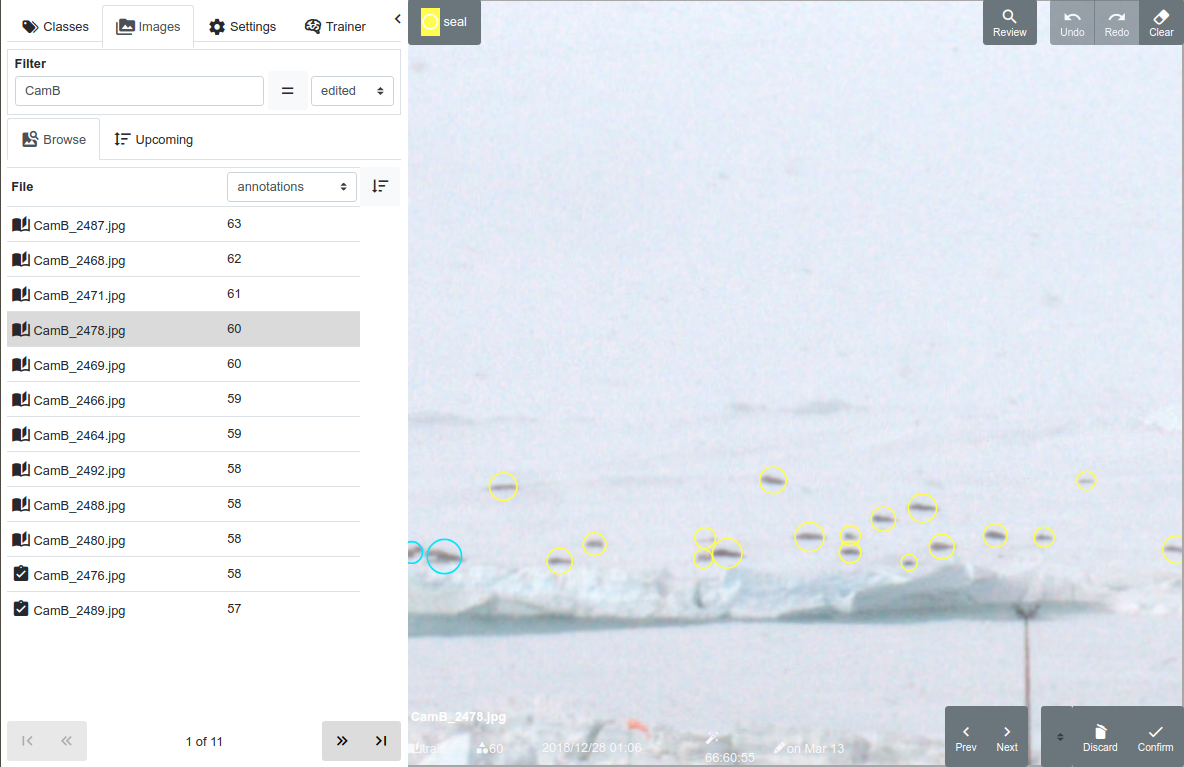
\includegraphics[width=1.0\linewidth]{figures/annotation/screenshots/sort_filter.png}
  \caption{Interface for sorting and filtering a dataset, here showing a search for ``CamB'', restricted to edited images and ordered by number of annotations}  
  \label{fig:sorting_filtering}
\end{figure}

In addition to the metrics used for example selection, I found it useful to provide ways for a user to filter and rank images according to various criteria. An example of this is shown in figure~\ref{fig:sorting_filtering}.

Filtering methods include:

\begin{itemize}
    \item {\bf Image usage } \par
Find images intended for testing, training or validation; unseen or annotated images. Uses include finding unseen images to visually evaluate performance, or validation images and reviewing training images.

\item {\bf Search by sub-string.} \par

Fuzzy matching is used to find images with names matching a query string. This is useful for cross-referencing external files or sorting by attributes present in a file-name such as an annotation month.

\end{itemize}

In future, this may include all kinds of other attributes such as image level attributes or the user who annotated the image.

Ranking criteria include:

\begin{itemize}
    \item {\bf Modification time.} \par
Order images by least recently modified.
    \item {\bf Image creation time. } \par
Select images by the time they were captured - useful for comparing images in time. One example is synchronising images taken concurrently from different streams, for example, seal counts at Scott Base captured by two different cameras.
    \item {\bf Validation or testing score. } \par
Order images used in validation or testing by the primary evaluation metric (for object detection this is the $AP_{COCO}$ in most cases, details in chapter~\ref{chap:object_detection}).
\end{itemize}

\section {Implementation}

\subsection{Server and client}

\begin{figure}[h!]
  \centering
  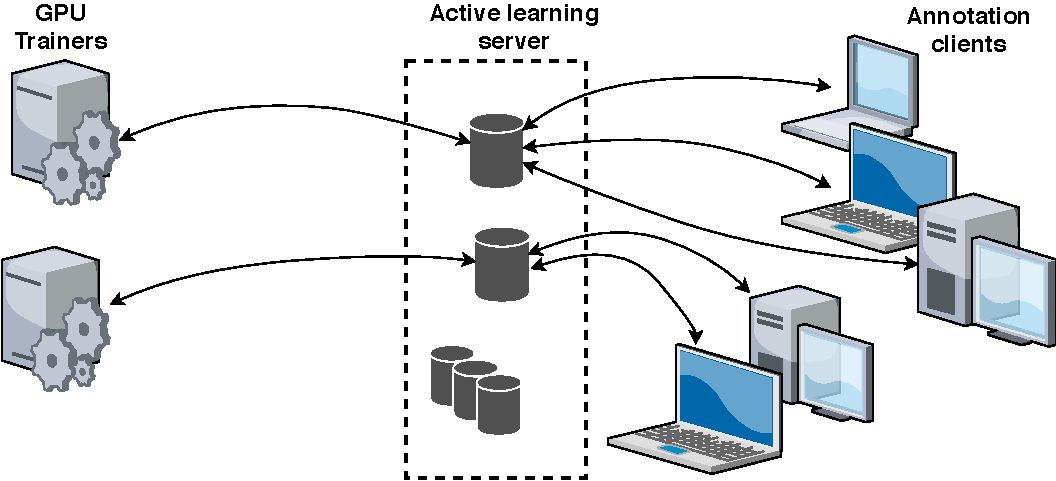
\includegraphics[width=1.0\linewidth]{annotation/connectivity.pdf}
  \caption{Connectivity of the annotation system}  
  \label{fig:connectivity}
\end{figure}

The system can be broken down into three parts running separately but communicating with each other (see figure~\ref{fig:connectivity}). The server sits in the middle and communicates with both trainers and clients, as well as storing data (image data, annotations and annotation history, trained models and annotations).

The main reason for splitting the server and trainer was initially for practical reasons with the client and server both written in \gls{GHC} Haskell, and the deep learning framework of choice being Pytorch \cite{Paszke2017}. The server and client are written in Haskell, the former running naively, the latter compiled to JavaScript using \gls{GHCJS}. The interface uses a \gls{SVG} for display, but in future, I plan to switch to \gls{HTML} canvas for faster rendering in a wider variety of browsers and resolve issues with displaying hundreds of annotations at once.

Splitting server and trainer also provides some advantages. It allows the server to act as a portal through which users can work on several datasets. One or many trainers can be shared concurrently or time-shared without having to run new instances of the server. 

The current reality is more simple, a single trainer services the server and operates on a first come, first served basis. One dataset at a time is trained, until a period of inactivity (no images submitted for $ n $ training epochs). A trainer still services clients working on inactive datasets by providing detection (best models for each dataset are kept in \gls{CPU} memory), but trains on only one dataset at a time. 

Due to the nature of memory management on a \gls{GPU}, and the memory requirements of training, I interleave requests originating from clients and training. When a user selects an image, the first action taken is to query the trainer for a set of detections. It is, therefore, necessary to stop training temporarily, perform object detection inference on the image in question, and then resume training. In an attempt to mitigate the delay, a small number of frames are processed in advance according to the current image selection policy in use at the time. For larger images, the transmission and decoding of image data in the current system causes more significant visible delay than the response time to the object detection query.

In future, it would be an advantage to allow one or more \gls{GPU} processes to be dedicated to serving user requests, in the interests of reducing response time. Low response time is important especially to interact with video if skipping forwards and backwards in time (spanning potentially many frames at a time), so this can occur without unreasonable delay.

\begin{figure}[h!]
  \centering
  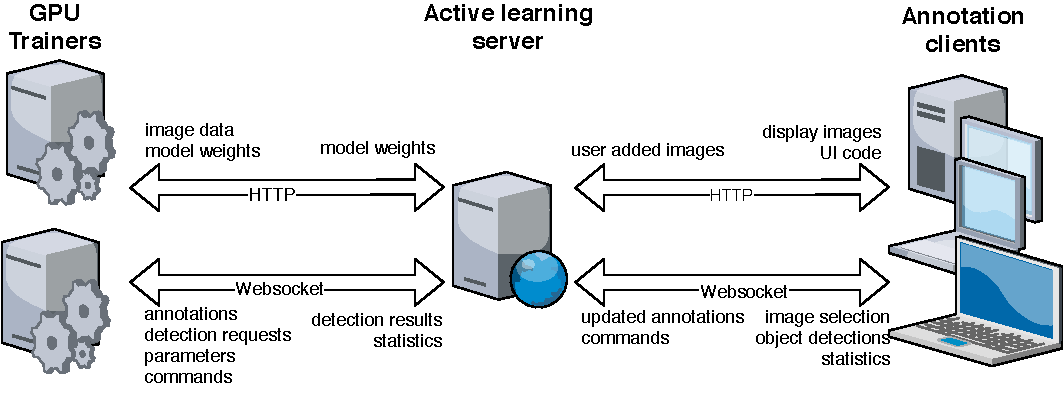
\includegraphics[width=1.0\linewidth]{annotation/data_flow.pdf}
  \caption{Data flow between services for the annotation system}  
  \label{fig:data_flow}
\end{figure}

An illustration of the data flow which occurs between different parties can be seen in figure~\ref{fig:data_flow}. Large binary data is shared using \gls{HTTP}, for example, model weights and images are distributed this way. Other data is communicated over WebSocket connections using \gls{JSON} text. Examples of this include synchronising new annotations and image statistics, which are continually updated to the client for the example selection in active learning.

Image data is stored on the server and transmitted as required to the trainer and the client. Images are sent to the client for viewing and inspection, and to the trainer for training and cached for more efficient loading. 

Models are stored on the server and requested by the trainer as required, for example, when starting training on a dataset, the trainer requests the previously stored model weights. The trainer also caches copies of weights (as required) of recently used models for inference as required by the client for every image opened. Given the large size of data involved in transmitting large images, and also updating model weights, it is crucial for the server to have a fast connection to the trainer.

\subsection {User interface}

I provide a web interface for the following reasons:

\begin{enumerate}
    \item Easy distribution
\end{enumerate}
Any system with a web browser can be used as a client. A web interface sidesteps difficulties with hardware requirements (a modern \gls{GPU}) and difficult to install software dependencies typically required to run \gls{CNN}s at a reasonable speed.
\begin{enumerate}[resume]
    \item Local GPU not required
\end{enumerate}
By running the trainer on another system, anyone can use the system without requiring a local GPU. One of the problems with usability, from my earlier work, was that GPU intensive tasks running on the same computer ruin the responsiveness of a user interface. To my knowledge, there is no good way to run a heavy \gls{GPU} intensive processing task at a low priority so that the user interface remains responsive.
\begin{enumerate}[resume]
    \item Enables collaborative annotation/crowdsourcing
\end{enumerate}
A web interface enables a straightforward extension to use for more substantial scale annotation with multiple users annotating the same dataset. An example can be seen in~\ref{fig:connectivity}, showing two groups of users operating on the same datasets.


The trade-off for a web interface is in performance, as it prevents doing computationally heavy calculations on the client side, especially for loading and processing large images. For this work, there is no such difficulty. With newer web technologies such as WebAssembly \cite{Haas2017}, it is possible to run code at near-native speeds in a browser and WebGL shaders for GPU programming.

\section{Current state}
\label{sec:current_state}

The current state of the system is mostly a working prototype. While it is already robust for use if set up on a server, the documentation for setting it up are sparse.  Key features such as support for setting up new datasets and many training parameters are not exposed to the user interface. A first step will be to provide simple methods for deployment on a cloud service with a set of images or videos, as well as providing easy methods for downloading and using trained models (and annotations).


\section{Future work}
\label{sec:design_future_work}

There exists a huge variety of potential scope for future work, including development. Some of the planned and potential ideas are listed here.

\subsection{Ensemble training and uncertainty estimation}

There exist a number of uncertainty measures, specifically developed for object detection, based on Bayesian \gls{NMS} \cite{Harakeh}, test time augmentation {Wei2018} and, of particular interest, ensembles \cite{Le2018}. Some discussion of this is in section~\ref{sec:example_selection}. 

K-fold cross-validation is proposed as a future method to improve data usage. It can be used for ensemble-based predictions on new images with uncertainty estimation, unbiased reviewing and machine-assisted verification to check for mistakes, and enhanced accuracy in testing by testing against the full dataset.

In conflict with our desire to use high-resolution images for annotation clarity, ensembles, example selection, and interface responsiveness would all benefit from the use of lower resolution images. More experimentation is necessary to determine the best tradeoff, which seems likely to depend on the dataset.

\subsection{Domain specific applications, counting wildlife}

One promising application for \gls{VBA} has been in counting wildlife, see sections~\ref{sec:case_penguins}~and~\ref{sec:case_seals}, where the annotation tool has been used for verified counting of Antarctic wildlife. Several limitations were discovered, such as efficiency issues with the user interface in the presence of very large numbers of annotations, and the difficulties created by the artificial splitting of images. Addressing efficiency is very straightforward, but a way of allowing the user to divide up very large images would seem beneficial.

Several metrics and image selection heuristics were added to attempt to aid experimentation with time series images. Expanding on these heuristics and providing better methods for exploring and sorting images would be beneficial for studying time series. Adding image level classification would also be useful for sorting and managing datasets. For example, automatically discarding images with poor visibility would be possible if discarded images are labelled and used for learning.

\subsection{Higher level forms of object detection}

\begin{figure}[h!]
\begin{subfigure}[t]{0.5\linewidth}
  \centering
  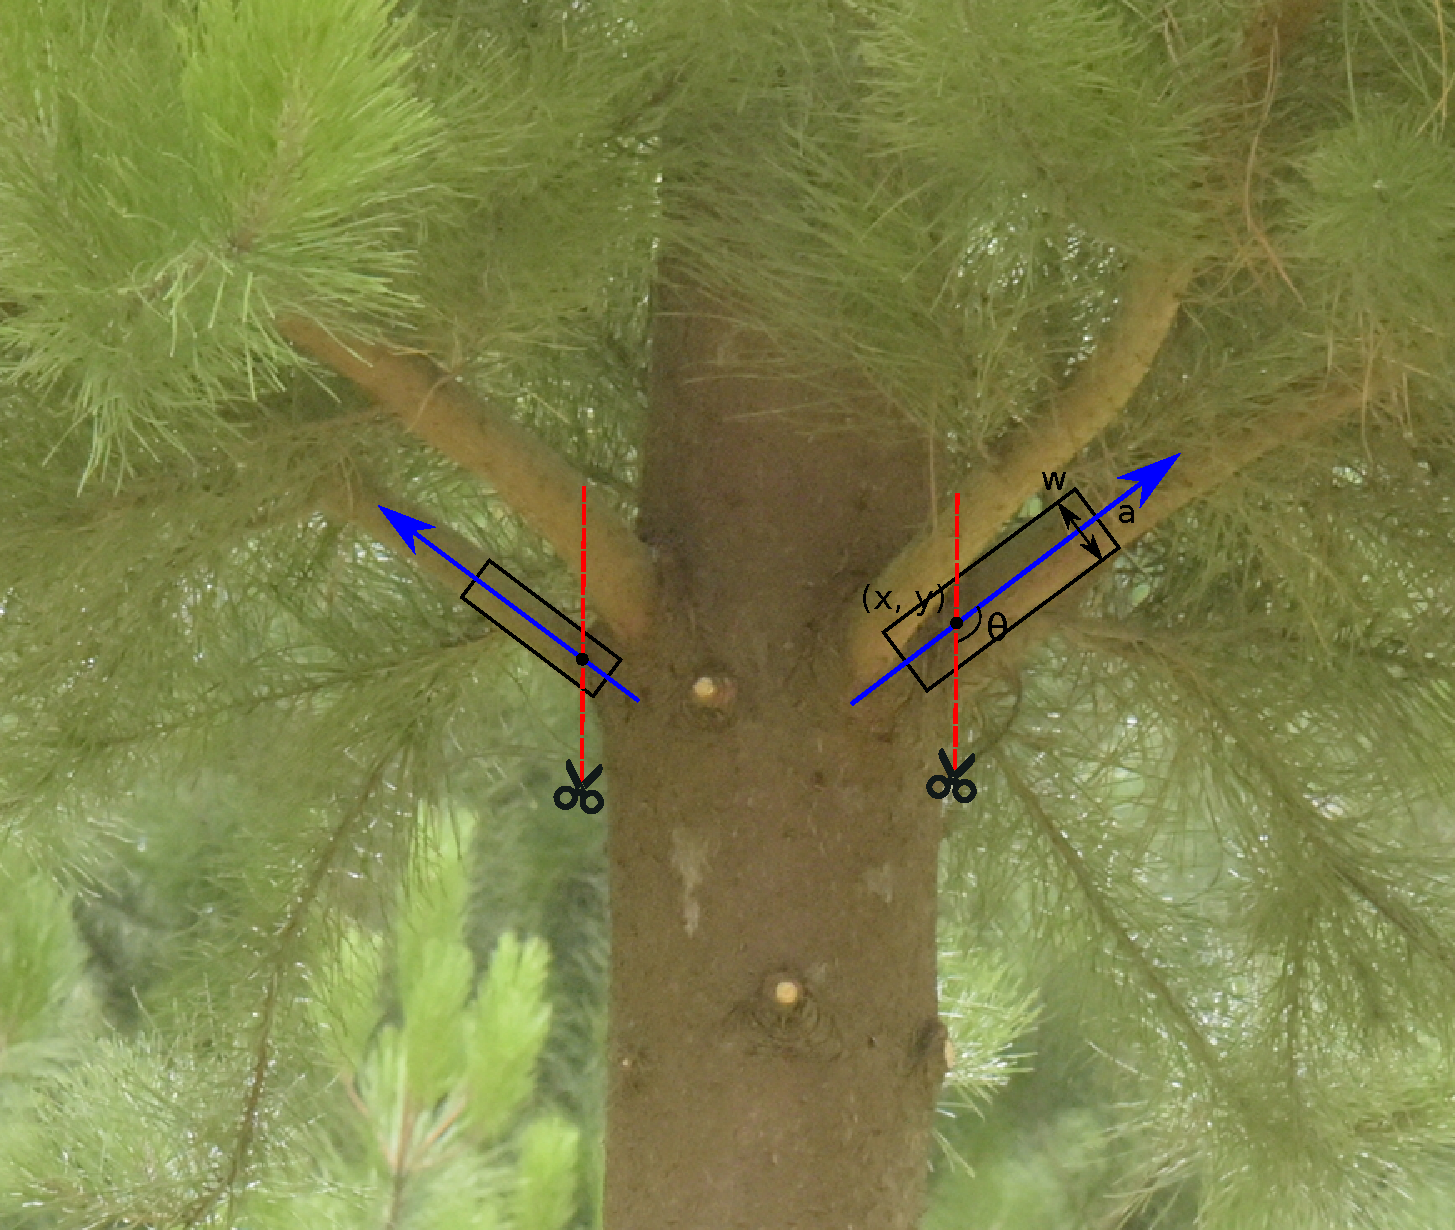
\includegraphics[height=0.25\textheight]{figures/future/tree_cutpoint.pdf}
  \caption{} 
\end{subfigure}%
\begin{subfigure}[t]{0.5\linewidth}
  \centering
  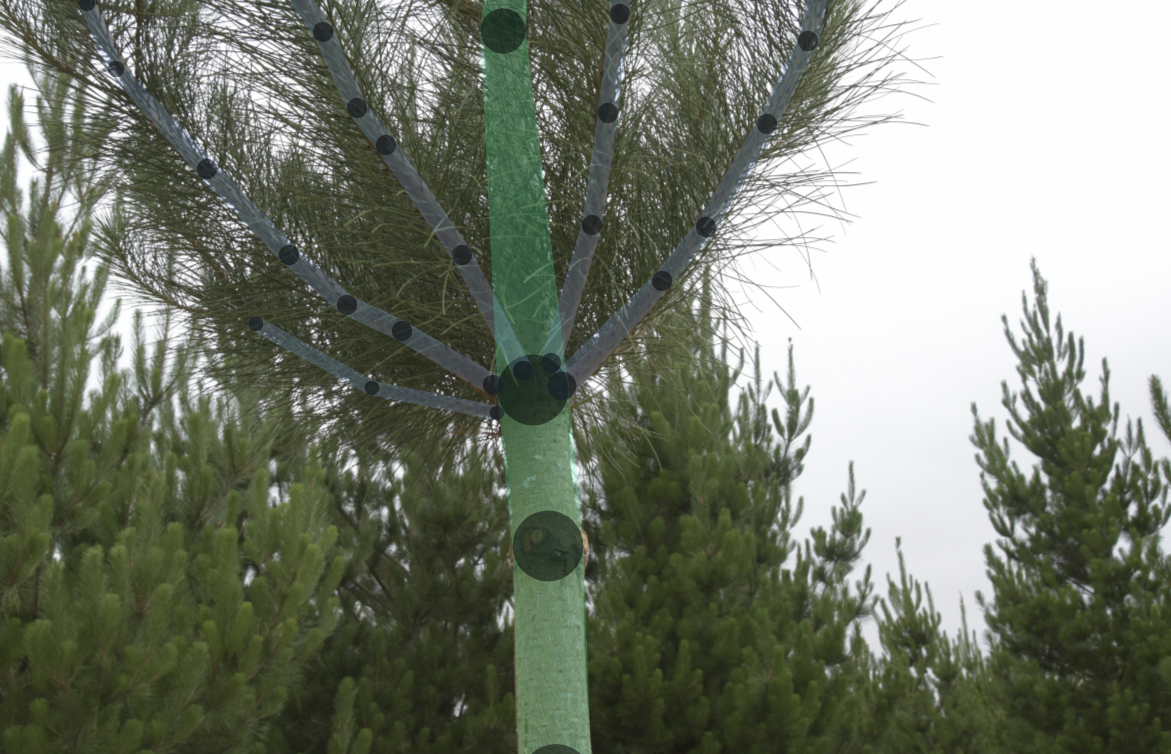
\includegraphics[height=0.25\textheight]{figures/future/tree_branches.jpg}
  \caption{} 
\end{subfigure}
\caption{Ongoing work into annotating trees in (a) cut-point detection, showing the parameters required to detect (and annotate) a cut point: the cut plane, centre point, branch angle, branch width (b) tree structure skeleton extraction, using piecewise lines with widths specified at control points (circles on the image) }
\label {fig:future_trees}
\end{figure}

Bounding boxes have limits for object detection; they only very loosely fit an object, and some objects cannot be described well by bounding boxes at all. Tree branches are fit by bounding boxes very poorly; they're very long, and it's not always clear where they start and stop. Future work will focus on other kinds of object detection, and the ability to pick the type for the task at hand.

Recent work in object detection \cite{Zhou2019} or \cite{Law2018}, both successors to the RetinaNet detector \cite{Wang2017} used in this work, have shown that both the anchor box approach and \gls{NMS} is unnecessary. In \cite{Zhou2019}, local maxima in a single heat map are used to detect objects, and all other parameters are regressed, allowing for the simple extension to a range of different types of object detector by regressing different properties.

The branches dataset used as an example in this work, is a trial for detecting cut positions. Figure~\ref{fig:future_trees} shows two directions in the annotation of tree structures, cut point estimation and skeletal extraction for robotic pruning applications. Skeleton estimation on tree structures can be adapted from methods used for road network extraction \cite{Li2018}, shape estimation \cite{Jiang2019a} or polygon extraction \cite{Acuna2018}, and can work well within the \gls{VBA} approach.

\subsection{Annotating uncertainty}

In future, the ability to annotate images based on uncertainty may be a useful approach, as a means of calibrating confidence and for weighting examples in the training process. As opposed to epistemic uncertainty, aleatoric uncertainty can be estimated directly (by a \gls{NN}, for example, by regression).  

This kind of uncertainty annotation may also be useful in weighting training loss, where the network can place more weight on hard, yet unambiguous examples. The use of Focal Loss means that examples which fail to classify well are weighted much more highly. If these examples are ambiguous because of shadow or lack of resolution - their contribution to the training is noise.

Hard examples are often cited as being the most useful for an object detector, but if the hard examples are not really hard examples, because they are also visually ambiguous or uncertain (high aleatoric uncertainty) then their usefulness as a learning target might be less, but still possesses value for use in validation and calibration.



\subsection{User verification and testing}
\label{sec:user_verification}

The risk of algorithmic bias brings into question the quality of a dataset annotated with a \gls{VBA} system.  To combat algorithmic bias when a human annotator becomes fatigued, it is proposed that a certain level of \emph{generated} mistakes can be included. The user may be forced to fix the error before they can continue, or statistics from fixing added errors may be used as a measure of the user's trustworthiness. Examples of generate mistakes include false positives, false negatives by removing very high confidence detection, or localisation errors by transform box of high confidence detection. 


\subsection{Software improvements}

There is a range of general software improvements to improve usability and prepare for release to a broader audience. 

\subsubsection {Removal of thresholds}
In the future, attention will be placed on making the annotation process more streamlined with less manual intervention required. Determining thresholds more automatically, or automated calibration using validation will be a focus.

\subsubsection {Improve rendering efficiency}
The user interface will switch rendering to a canvas based renderer from the current SVG rendering. This is needed to run on a wider variety of browser, and improve performance for situations where hundreds or thousands of annotations are present on a single image.

\subsubsection {Restricted annotation interface}
Splitting the user interface into an annotation interface and a supervisory interface will be necessary to support multi-user annotation. The annotation interface will be purely for annotation and has few settings, whereas the supervisory interface is much like the current interface, with full control over the process and with the ability to monitor others.

\subsubsection {Deployment to cloud services}
Currently, setting up a server and training processes is a manual job, and although it is simple to access through the web interface once setup, more general usage will be enabled through providing scripts to deploy the software (along with images) to cloud services such as \gls{AWS}. 

\subsubsection {Exposing parameters and settings}
 Many object detection model and training settings in the current implementation are still stored on the training process and not controlled centrally. It is planned to expose those parameters through the user interface, and importantly, be able to adapt to those training parameters (even if it requires restarting the training).

\subsubsection{Visualisations and metrics in the interface}

The current approach to providing metrics to a user is to run an instance of Tensorboard next to the training process. However, an alternative solution will be sought, which means logs can be stored centrally with the rest of the data, as opposed to Tensorboard log files.

